% 曲边梯形的面积
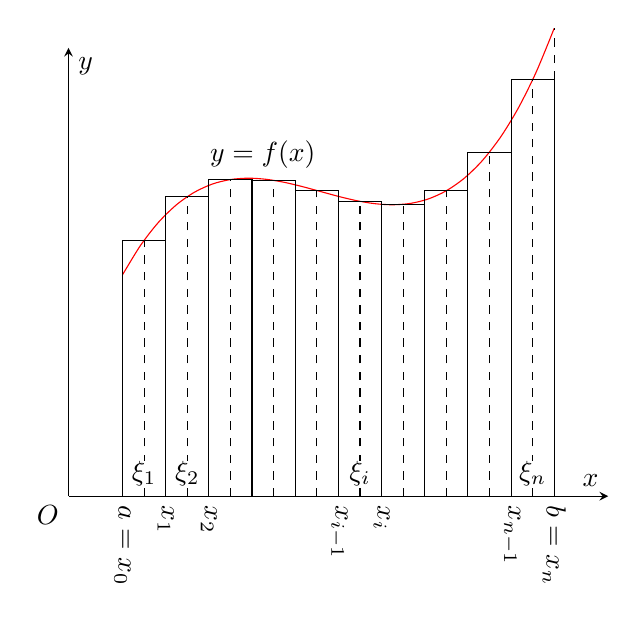
\begin{tikzpicture}[scale=1]
  \begin{axis}[clip=false,xmin=0, xmax=5,ymin=0,ymax=5, grid=none,
    xtick=\empty, ytick=\empty, axis lines=middle,
    smooth, xlabel={$x$}, ylabel={$y$}]

    % 曲线: ((x-2)**3-(x-2)**2-x)/4.0 + 4
    \addplot[draw=red,domain=0.5:4.5] {(x-2)^3/4 - (x-2)^2/4 - x/4 + 4};

    \node [above] at (1.8,3.55) {$y=f(x)$};

    \draw (0.5,0) rectangle (0.9,2.853); \draw [dashed] (0.7,0) -- (0.7,2.853);
    \draw (0.9,0) rectangle (1.3,3.34); \draw [dashed] (1.1,0) -- (1.1,3.34);
    \draw (1.3,0) rectangle (1.7,3.531); \draw [dashed] (1.5,0) -- (1.5,3.531);
    \draw (1.7,0) rectangle (2.1,3.522); \draw [dashed] (1.9,0) -- (1.9,3.522);
    \draw (2.1,0) rectangle (2.5,3.409); \draw [dashed] (2.3,0) -- (2.3,3.409);
    \draw (2.5,0) rectangle (2.9,3.288); \draw [dashed] (2.7,0) -- (2.7,3.288);
    \draw (2.9,0) rectangle (3.3,3.255); \draw [dashed] (3.1,0) -- (3.1,3.255);
    \draw (3.3,0) rectangle (3.7,3.406); \draw [dashed] (3.5,0) -- (3.5,3.406);
    \draw (3.7,0) rectangle (4.1,3.837); \draw [dashed] (3.9,0) -- (3.9,3.837);
    \draw (4.1,0) rectangle (4.5,4.644); \draw [dashed] (4.3,0) -- (4.3,4.644); \draw [dashed] (4.5,4.644) -- (4.5,5.219);

    \node [right, rotate=-90] at (0.5,0) {$a=x_0$}; \node [above,fill=white,inner sep=0.2] at (0.7,0.1) {$\xi_1$};
    \node [right, rotate=-90] at (0.9,0) {$x_1$}; \node [above,fill=white,inner sep=0.2] at (1.1,0.1) {$\xi_2$};
    \node [right, rotate=-90] at (1.3,0) {$x_2$};
    \node [right, rotate=-90] at (2.5,0) {$x_{i-1}$}; \node [above,fill=white,inner sep=0.2] at (2.7,0.1) {$\xi_i$};
    \node [right, rotate=-90] at (2.9,0) {$x_i$};
    \node [right, rotate=-90] at (4.1,0) {$x_{n-1}$}; \node [above,fill=white,inner sep=0.2] at (4.3,0.1) {$\xi_n$};
    \node [right, rotate=-90] at (4.5,0) {$b=x_n$};

    % 原点
    \node [below left] at (0,0) {$O$};
  \end{axis}
\end{tikzpicture}
